\documentclass{acm_proc_article-sp}
\usepackage{url}
\usepackage{graphicx}
\begin{document}
\title{Sheetmusic: Making music from spreadsheets}
\numberofauthors{1}
\author{
\alignauthor
Thomas Levine\\
       \affaddr{csv soundsystem}\\
       \email{\_@thomaslevine.com}
}
\date{6 March 2014}
\maketitle
\begin{abstract}
The spreadsheet is an intuitive paradigm for the expression of musical
scores. I'll discuss how you can turn data into music with our Sheetmusic
software and show examples of how csv soundsystem turns spreadsheets
into data-driven music videos.
\end{abstract}
\section{Introduction}
In our production of data-driven music videos, we have recognized a need
for data analysis software and music software to be more strongly integrated.
We wanted a more seamless transition between modeling and music, and we
wanted it to be easier for data analysts to work with music. We have
developed tools like Sheetmusic (\url{http://github.com/csv/sheetmusic})
to bridge this gap.

\section{How it works}
We've found that the tabular representation of data aligns very well with
typical representations of music. Sheetmusic works by mapping these two
concepts to each other.

We can think of data tables as collections of similar things, with the
same sorts of information being collected about each thing. In tidy data
tables \cite{tidydata} each row corresponds to an observation (a thing),
and each column corresponds to a variable. We add more rows to the table
as we observe more things, and we add more columns to the table as we
collect more information about each thing.

We can think of music as a composition of many different sounds over time,
with sounds coming from many different instruments. In musical scores
we represent time as movement from left to right, and we represent different
instruments by different staves (stacked on top of each other).
The staff becomes wider as the song gets longer, (They are often spread
across multiple pages.) and we add more staves as we add more instruments.

If we constrain the manner of data and of music, we can losslessly convert
between the data table concept and the musical staff concept. As an example,
let's look at a passage from Chopin's \'Etude Op. 10, No. 1. \cite{chopin}.
Figure \ref{sheet} represents it in ordinary sheet music.

\begin{figure}
\label{sheet}
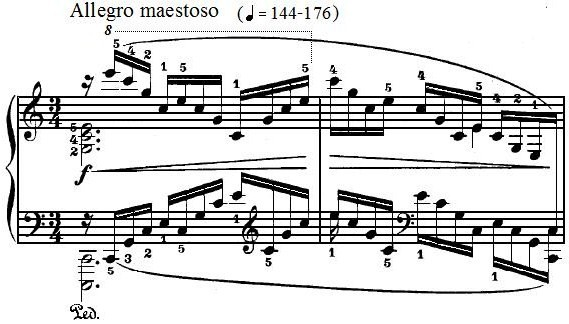
\includegraphics[width=\columnwidth]{chopin.png}
\caption{Chopin's \'Etude Op. 10, No. 1. as ordinary sheet music}
\end{figure}

Table \ref{table} displays it as a data table as comma-separated values.
(Well almost; it doesn't include the two chords of dotted half notes.)

\begin{table}
\label{table}
\centering
\begin{tabular}{c c} \hline
Left Hand&Right Hand\\ \hline
   (NA)  &   (NA)\\
    C2   &    E6\\
    G2   &    C6\\
    C3   &    G5\\
    E3   &    C5\\
    C3   &    E5\\
    G3   &    C5\\
    C4   &    G4\\
    E4   &    C4\\
    C4   &    G4\\
    G4   &    C5\\
    C5   &    G5\\
    E5   &    C6\\
    C5   &    G5\\
    G4   &    C5\\
    C4   &    G5\\
    E4   &    C5\\
    C4   &    G4\\
    G3   &    C4\\
    C3   &    E4\\
    E3   &    C4\\
    C3   &    G3\\
    G2   &    E3\\
    C2   &    C3\\ \hline
\end{tabular}
\caption{Chopin's \'Etude Op. 10, No. 1. as a data table}
\end{table}

Rather than composing music as traditional sheet music,
we can use a table-editing program of our choice to compose
this sort of table.

\section{How to use it}
Sheetmusic is implemented as a JavaScript function that loads data
from a Google Spreadsheet. Given the URL of a spreadsheet, Sheetmusic
downloads the spreadsheet contents and plays them in a browser.

The spreadsheet is organized as follows. Each column corresponds
to a musical track, and different tracks can have different music instruments.
Row corresponds to a beat (of time).
Each cell contains the frequency of sound to be played, represented
either as a number (Hertz) or in scientific notation (C4, D4, \&c.).

Sheetmusic accomplishes the playback of music, and this leaves
the data analyst to use conventional spreadsheet approaches for
composing music. For example, the following function can be used
to produce a major scale in a spreadsheet column.
\begin{verbatim}
# For example: ionian(440, 8)
function ionian(base, n) {
 var s = [0, 2, 4, 5, 7, 9, 11, 12]
 function freq(i) {
  return base*Math.pow(2,(Math.floor(i/12)+s[i])/12)
 }
 var scale=[]; for (var i=0; i<n; i++) scale.push(i)
 return scale.map(freq)
}
\end{verbatim}
Once you have a major scale in one column, you can easily make
chords with a spreadsheet function like this.
\begin{verbatim}
=A1*2^(4/12)
\end{verbatim}
If you put this in cell B1, A1 and B1 will form a major third interval
\cite{majorthird}.
You can read more about the determination of frequencies on Wikipedia \cite{piano}.

\section{Why make data-driven music}
We created sheetmusic and similar tools out of a need to produce
data-driven music, but I neglected to explain why we needed to do
that. Here are some of the uses that we have found for data-driven
music and music videos.

\subsection{Analyzing complex data}
Now that we're collecting so much data, we are reaching the limits of
data visualization. When produced and interpreted by capable people,
a good data visualization can represent about eight different variables.
If we want to visualize more variables than that, we must settle for
a reduced version of the data. By leveraging the sense of sound,
we expand our sensory bandwidth and enable the representation of
higher-dimensional data.

In the long term, we really need to gastronomify (turn into food)
data in order to experience them with all of the senses.
Unfortunately, that isn't feasible right now;
until we develop cheaper taste and smell APIs, we are stuck with what we have
on our smartphones, laptops, \&c., which is vision, hearing and touch. We need
to make data music videos in order to make the most of these tools.

\subsection{Reaching young people}
Combining data with music may also appeal to a younger audience.
According to the fictional eleven-year-old Emma Gertlowitz whose crush
recently switched from Justin Bieber to Nate Silver \cite{emma},
``[S]tatisticians are the new sexy vampires, only even more pasty.''
This example is just part of a larger trend: data is "in".

The White House used the appeal of data and music to advertise the State
of the Union Address; they published a video advertisement to YouTube that
used pie charts and dubstep, presumably to appeal to a younger audience \cite{whitehouse}.

\subsection{Education}
I find that a major hurdle in the understanding of quantitative disciplines
is an intuition of how to break complex concepts into discrete numbers.
I find that mapping numbers to things other than graphs gets people thinking
a bit more about what the numbers mean.

\subsection{People who can't see}
Data visualizations are typically not accompanied by an equivalent
alternative for people who can't see. We can redundantly express data
across multiple senses in order that people of varied ability can all
experience a particular data analysis.

\bibliographystyle{abbrv}
\bibliography{spreadsheets}
\balancecolumns
\end{document}
